\subsection{Main Deployment} \label{sec:mainDeployment}
In this section I will discuss the desired system and what was actually implemented. The shortcomings and their reasons are discussed in the next section.
\Cref{fig:implementationSetup} shows the desired system setup.
\begin{figure}
    \centering
    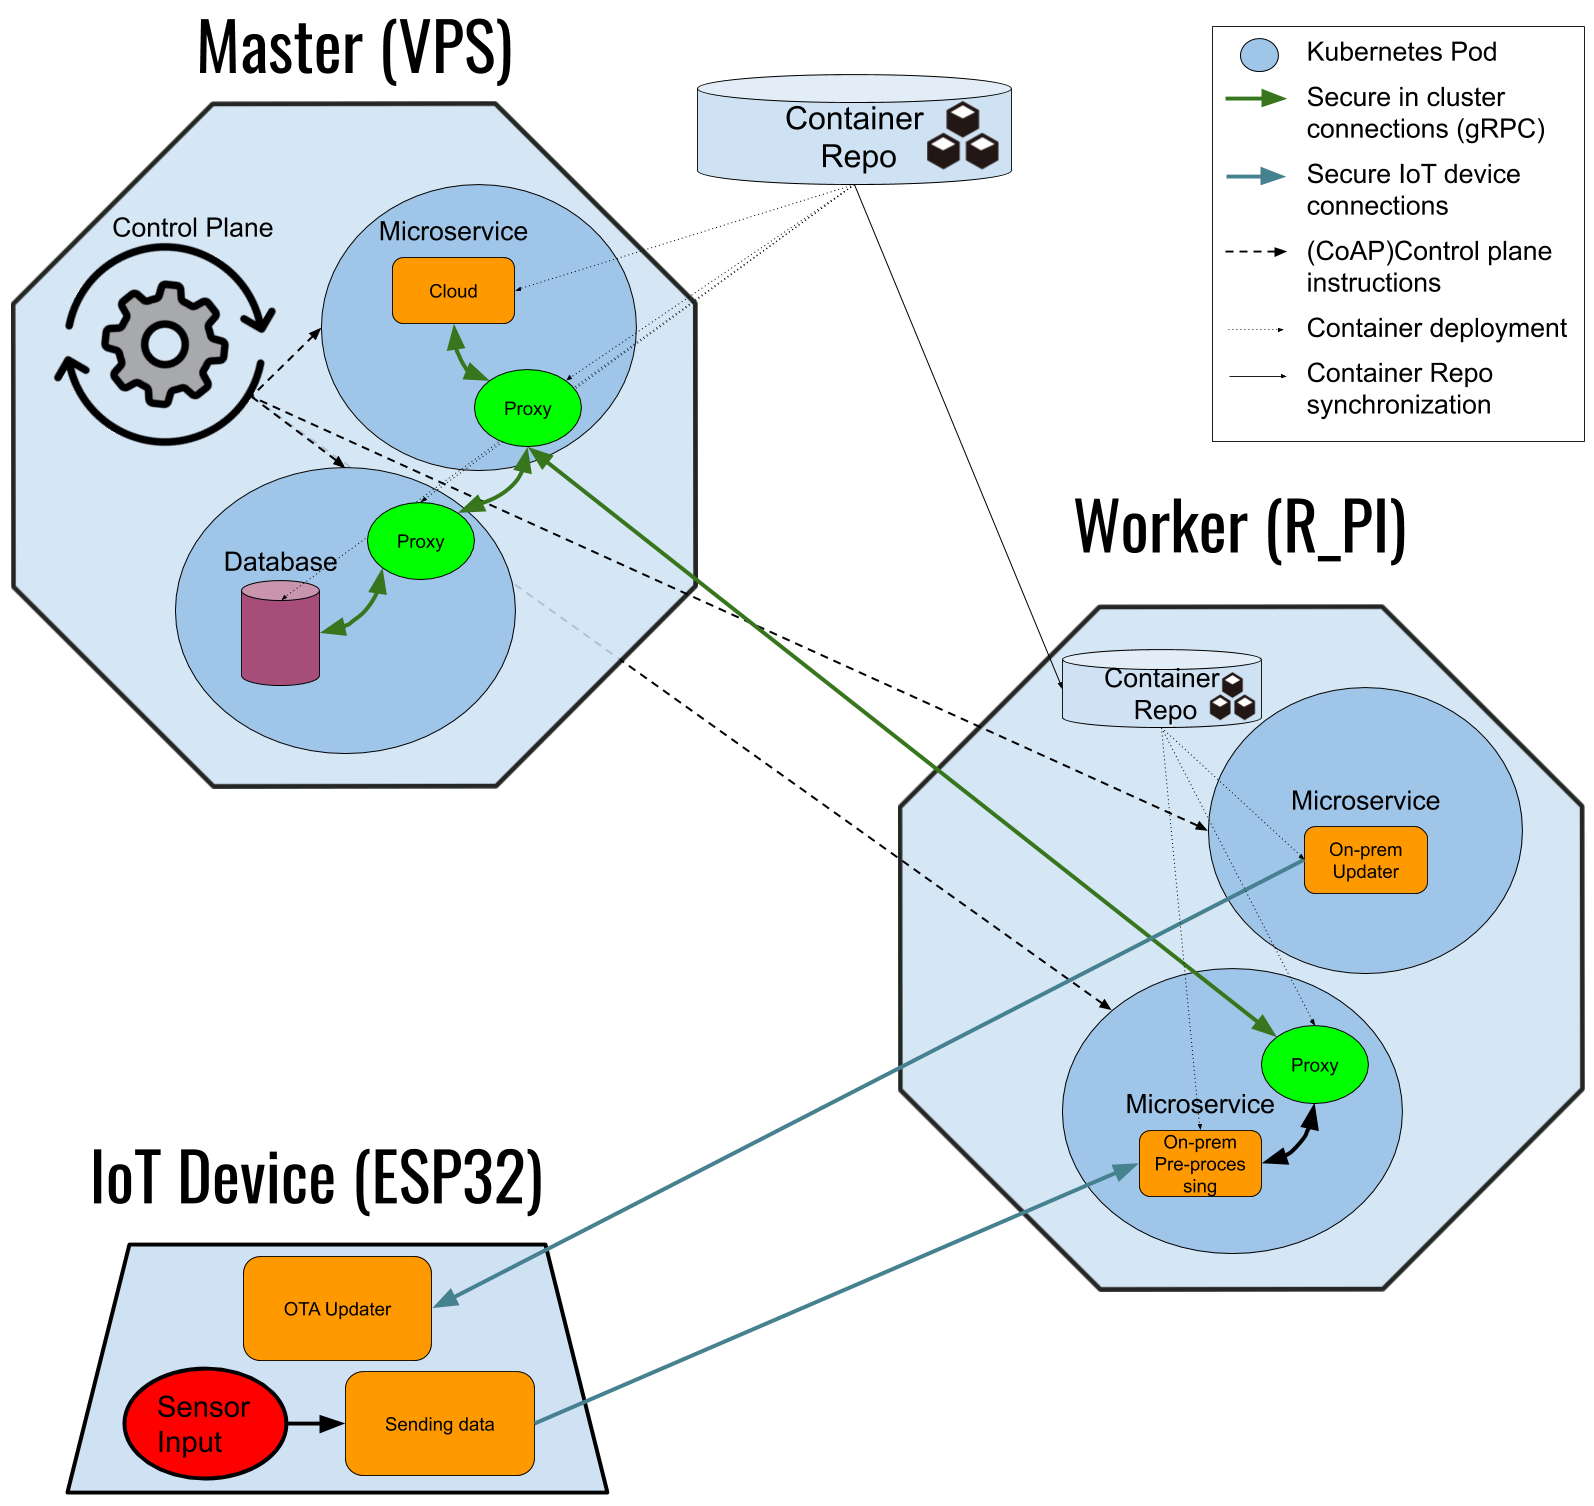
\includegraphics[scale=0.25]{figures/implementationSetup.png}
    \caption{The desired system setup for this implementation.}
    \label{fig:implementationSetup}
\end{figure}
The cloud and edge run Kubernetes and the IoT device runs RTOS with Arduino. All services running inside containers are programmed in Go and the IoT service in the Arduino programming language. 
The master node in the cloud is in control of the system and runs on a virtual private server and not on bare metal as recommended by industry experts. VPS make management easier and with recent improvements of the hypervisor software performance is not much worse than bare metal deployments. Also, performance on the master is not of major interest in this thesis. The master also includes two pods, one is a stateless service to process the edge data and the other one is a distributed database. Both include an envoy proxy from Istio, which functions as the pods internal gateway. This means all network connections go through this service and can be modified. It also enables autmotic mesh internal communication in gRPC and TLS encryption. Both pods have toleration to the masters taint of no scheduling. The containers are pulled from an outside registry, the Docker Hub.\\
The worker node runs on an on-prem deployed Raspberry Pi and is instrumented from the master. It is labeled as an edge node and contains two pods, one for normal (business related) communication with the IoT device, an esp32, and one pod for OTA updates which is only deployed when an new update is scheduled. Both have the \textit{nodeAffinity} set to the edge tag. The worker keeps a synchronized local container registry of the cloud with the repositories used on on-prem. It is part of the orchestration network to enable future changes to it. The business related microservice does only light preprocessing of the sensor data and does not contain a database. The pod contains an Istio proxy to enable automatic efficient and secure communication with the the cloud. The communication with the IoT device is over CoAP and encrypted with DTLS. \\
Finally, the IoT device is a esp32. It has two logical services, monitoring the sensor input and sending it to the edge (1) and an OTA update service (2). Because of memory and RTOS restrictions, they run in the same code base. Due to simplicity, in this project a simple button 